% Multiple Choice Question 27 to 28 (2 questions)

% \par\noindent\rule{0.75\textwidth}{0.5pt} 
\textbf{See the instruction for questions \inteval{\value{question}+1} to \inteval{\value{question}+2}.} 

\begin{center}
    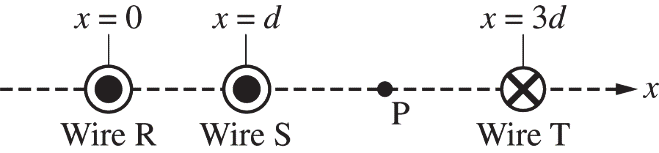
\includegraphics[scale=0.3]{images/img-013-025.png}
\end{center}

Three long, current-carrying wires are shown in the cross-sectional view above. The currents in wires $\mathrm{R}$ and $\mathrm{S}$ are out of the page, and the current in wire $\mathrm{T}$ is into the page. The currents in the wires have equal magnitude, and the wires are in the positions shown. Point $\mathrm{P}$ is halfway between wires $\mathrm{S}$ and $\mathrm{T}$.

\begin{questions}
\setcounter{question}{26}

% Multiple Choice Question 27
\question
If $B_{\mathrm{S}}$ is the magnitude of the magnetic field at point $P$ due to wire $S$, which of the following gives the magnitude and direction of the magnetic field at point P due to all three wires?

\tabto{0.75cm} \underline{Magnitude}
\tabto{4.00cm} \underline{Direction}

\begin{choices}
    \choice $B_{\mathrm{S}} / 2$   \tabto{3.25cm} Top of the page 
    \choice $B_{\mathrm{S}} / 2$   \tabto{3.25cm} Bottom of the page 
    \choice $B_{\mathrm{S}}$       \tabto{3.25cm} Top of the page 
    \choice $5 B_{\mathrm{S}} / 2$ \tabto{3.25cm} Top of the page 
    \choice $5 B_{\mathrm{S}} / 2$ \tabto{3.25cm} Bottom of the page 
\end{choices}

% Multiple Choice Question 28
\question
To which of the following locations, if any, could wire $S$ be moved so that the total magnetic force exerted on it by the other two wires is zero?

\begin{choices}
    \choice $-d < x < 0$ 
    \choice $0 < x < d$ 
    \choice $d < x < 2d$ 
    \choice $2d < x < 3d$
    \choice There is no position in the vicinity of the wires at which the magnetic force on wire S would be zero.
\end{choices}

\end{questions}
